\documentclass{beamer}

\usepackage{txfonts}
\usepackage{hyperref}

\hypersetup{colorlinks=false,linkbordercolor=red,linkcolor=green,pdfborderstyle={/S/U/W 1}}

\addtobeamertemplate{navigation symbols}{}{ \hspace{1em}    \usebeamerfont{footline}%
    \insertframenumber / \inserttotalframenumber }

\geometry{papersize={12.8cm,12cm}}
\usepackage{lipsum}

\makeatletter
\newenvironment<>{contdproof}[1][\proofname]{%
    \par
    \def\insertproofname{#1\@addpunct{.}}%
    \usebeamertemplate{proof begin}#2}
  {\usebeamertemplate{proof end}}
\makeatother


\setbeamertemplate{theorems}[numbered]

\newtheorem*{nonumdefinition}{Definition}
\newtheorem*{nonumproblem}{Problem}
\newtheorem*{nonumremark}{Remark}
\newtheorem*{nonumexample}{Example}
\newtheorem*{nonumproposition}{Proposition}
\newtheorem{proposition}[theorem]{Proposition}


\usepackage{tikz}
\newcommand*\mycirc[1]{%
  \tikz[baseline=(C.base)]\node[draw,circle,inner sep=.7pt](C) {#1};\:
}


\newcommand\myheading[1]{%
  \par\bigskip
  {\color{blue}{\large #1}}\par\smallskip}

%\usetheme{Warsaw}
%\usetheme{Berkeley} %sample 1
\usetheme{Berlin} % sample 2
%\usetheme{AnnArbor} % sample 3

\let\otp\titlepage
\renewcommand{\titlepage}{\otp\addtocounter{framenumber}{-1}}



\title{Lecture 2 : Counting Techniques}
\author{}
\date{}


\begin{document}
\begin{frame}[plain]
\titlepage
\end{frame}

\begin{frame}
\frametitle{2.3 The Three Basic Rules}

\myheading{1. The Product Rule for Ordered Pairs and Ordered $k$-tuples}

Our first counting rule applies to any situation in which a set consists of \underline{ordered} pairs of objects $(a,b)$ where a comes from a set $B$.

In terms of pure mathematics the \underline{Cartesian product} $A\times B$ is the set of such pairs
$$
A\times B=\{(a,b) : a\in A, b\in B\}
$$ 
\end{frame}

\begin{frame}
\begin{nonumproposition}[text pg. 60]
If the first element of the ordered pair can be selected in $n_{1}$ ways and \underline{if for each of these $n_{1}$ ways} the second element can be selected in $n_{2}$ ways then the number of pairs is $n_{1}n_{2}$.
\end{nonumproposition}

Mathematically - If $\sharp(A)=n_{1}$ and $\sharp(B)=n_{2}$ then $\sharp(A\times B)=n_{1}n_{2}$.

There are analogous results for ordered triples etc.
$$
\sharp (A\times B\times C)=n_{1}n_{2}n_{3}
$$
\end{frame}

\begin{frame}
\begin{nonumexample}
How many ``words'' of two letters can we make from the alphabet of five letters $\{a,b,c,d,e\}$.
\end{nonumexample}

\begin{solution}
Note that order counts $ab\neq ba$.


There are two ways to think about the problem pictorially.

\myheading{1. Filling in two slots \underline{~} \underline{~}}

We have a choice of 5 ways to fill in the first slot and for each of these we have 5 more ways to fill in the second slot so we have 25 ways.
$$
\underline{5} \ \underline{5}=25
$$
\end{solution}
\end{frame}

\begin{frame}
\begin{solution}[Solution (Cont.)]
\myheading{2. Draw a tree where each edge is a choice}

\smallskip
\centerline{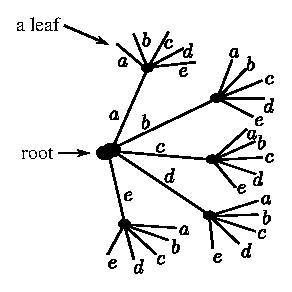
\includegraphics{figure/fig1.eps}}
\smallskip

The number of pairs is the number paths from the root to a ``leaf'' (i.e., a node at the far right).

In this case there are 25 paths.
\end{solution}

\begin{nonumproblem}
How many words of length 3?
\end{nonumproblem}
\end{frame}

\begin{frame}
\myheading{2. Permutations (pg. 62)}

In the previous problem the word $aa$ was allowed. What if we required the letters in the word to be distinct. Then we would get 2-permutations from the 5-element set $\{a,b,c,d\}$ according to the following definition.

\begin{nonumdefinition}
An \underline{ordered} sequence of $k$ \underline{distinct} objects taken from a set of $n$ elements is called a \underline{$k$-permutation} of the $n$ objects. The number of $k$-permutations of the $n$ objects will be denoted $P_{k,n}$.
\end{nonumdefinition}
\end{frame}

\begin{frame}
So \underline{order counts}

Let us return to our 5 element set $\{a,b,c,d,e\}$ and count the number of 2-permutations. 

It is best to think in terms of slots
$$
\underline{5}~\underline{4}=20
$$
There are 5 choices for the first slot but only 4 for the second because whatever we put in the first slot cannot be put in the second slot so $P_{2,5}=20$.

What is $P_{3,5}$?
\end{frame}

\begin{frame}
\begin{nonumproposition}[pg. 68]
$$
P_{k,n}=\underbrace{n(n-1)(n-2)\ldots(n-k+1)}_{k\text{~ terms}}
$$
\end{nonumproposition}

\begin{proof}
Fill in $k$ slots with no repetitions

\smallskip
\centerline{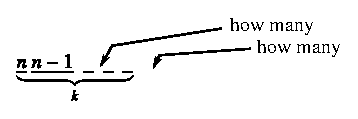
\includegraphics{figure/fig2.eps}}
\smallskip

Note that if we allowed repetitions we would get $n^{k}$
$$
\underbrace{\underline{n} \ \underline{n} \ \underline{n} \ \ \underline{~~} \ \underline{n}}_{k}
$$
\end{proof}
\end{frame}

\begin{frame}
There is a very important spacial case
$$
P_{n,n}=n!=n(n-1)(n-2)\ldots 3.2.1
$$
There are $n!$ ways to take $n$ distinct objects and arrange them in order.

\begin{nonumexample}
$n=3$, $\{a,b,c\}$
$$
\left.
\begin{array}{c}
abc\\
acb\\[3pt]
bac\\
bca\\[3pt]
cab\\
cba
\end{array}
\right\}\quad 3!=(3)(2)(1)=6
$$
When you list objects it is helpful to list them in dictionary order.
\end{nonumexample}
\end{frame}

\begin{frame}
\myheading{A Better Formula for $P_{k,n}$}

Here is a better formula for $P_{k,n}$.

\begin{nonumproposition}
$P_{k,n}=\dfrac{n!}{(n-k)!}$
\end{nonumproposition}

\begin{proof}
This is an algebraic trick
$$
\dfrac{n!}{(n-k)!}=\dfrac{n(n-1)\ldots (n-k+1)\overbrace{(n-k)(n-k-1)\ldots 3.2.1}^{(n-k)!}}{(n-k)!}
$$
So cancel the second part of the numerator with the denominator
$$
\dfrac{n!}{n-k+1}=n(n-1)\ldots (n-k+1)=P_{k,n}
$$
\end{proof}
\end{frame}

\begin{frame}
\myheading{The Birthday Problem}

Suppose there are $n$ people in a room. What is the probability $B_{n}$ that at least two people have the same birthday (eg., March 11)?

Let $s$ be the set of all possible birthdays for then $n$ people so
\begin{gather*}
\sharp (s) =(365)^{n}\\[4pt]
\underbrace{\underline{~~} \ \ \underline{~~} \ \ \underline{~~} \ \ \underline{~~} \ \ \underline{~~} \ \ \underline{~~} \ \ \underline{~~}}_{n\text{~people}}
\end{gather*}
(we ignore leap-years so this isn't quite right)
\end{frame}

\begin{frame}
Now let $A\subset s$ be the event that at least two people have the same birthday. So $A'$ = all the people in the room have different birthdays.

So
$$
B_{n}=1-P(A')
$$
Now what is $A'$? Order the people
$$
\dfrac{365}{1} \ \ \dfrac{364}{2} \ \ \dfrac{~~~}{3} \ \ \dfrac{~~~}{~~~} \ \ \dfrac{~~~}{~~~} \ \ \dfrac{365-n+1}{n}
$$
$\sharp (A')=P_{n},365$.

\medskip

So
$$
B_{n}=1-\dfrac{P_{n,365}}{(365)^{n}}
$$
\end{frame}

\begin{frame}
\myheading{Combinations}

There are many counting problems in which one is given a set of $n$ objects and one wants to count the number of \underline{unordered} subsets with $k$ elements.

An unordered subset with $k$ elements taken from a set of $n$ elements is called a $k$-combination of that set. The number of $k$-combinations is denoted $C_{k,n}$.

Which is bigger $C_{k,n}$ or $P_{k,n}$?

What is $C_{n,n}$?
\end{frame}

\begin{frame}
\begin{nonumexample}
$P_{2,3}=6$, $C_{2,3}=3$

$S=\{a,b,c\}$

\begin{center}
\begin{tabular}{c|c}
2 permutations of $S$ & 2 combinations of $S$\\
\hline
$ab$ \ \ $ba$ & $\{a,b\}$\\
$bc$ \ \ $cb$ & $\{b,c\}$\\
$ac$ \ \ $ca$ & $\{a,c\}$\\
\hline
\end{tabular}
\end{center}
Each two combination gives rise to 2. $2$-permutations.

So
$$
P_{2,3}=2C_{2,3}=(2)(3)=6
$$
\end{nonumexample}
\end{frame}

\begin{frame}
\myheading{A Formula for $C_{k,n}$}

\begin{nonumproposition}[pg. 64]
\begin{gather*}
P_{k,n}=C_{k,n}\cdot k!\text{~~ So}\\[3pt]
C_{k,n}=\dfrac{P_{k,n}}{k!}=\dfrac{n!}{k!(n-k)!}
\end{gather*}
\end{nonumproposition}

\begin{proof}
To make a $k$-permutation first make an unordered choose of the $k$-elements i.e., choose a $k$-combination, then, for each such choice arrange the elements in order (there are $P_{k,k}=k!$ ways to do this). So we here
$$
\sharp (k\text{-permutations})=\sharp(k\text{-combinations})-k!
$$
\end{proof}
\end{frame}

\begin{frame}
\myheading{More notation}

The binomial coefficient $\binom{n}{k}$ is defined by
$$
\binom{n}{k}=\dfrac{n!}{k!(n-k)!}
$$
This is because
$$
\underbrace{(a+b)^{n}=\sum\limits^{n}_{k=0}\binom{n}{k}a^{k}b^{n-k}}_{\text{The binomial theorem.}}
$$
So
$$
C_{k,n}=\binom{n}{k}
$$
We will use $\binom{n}{k}$ instead of $C_{k,n}$.
\end{frame}

\begin{frame}
\myheading{The toast problem}

When my wife and I were on a trip to Spain with our church we had 20 people at dinner. We all clinked (is this a genuine English word) our classes. I dazzled my friends by telling how many clinks there were.

Now you can answer this question -- how many?
\end{frame}

\begin{frame}
\myheading{More Problems}

\begin{enumerate}
\item How many 5 card poker hands are there?

\item How many 13 card bridge hands are there?
\end{enumerate}
Lastly
\begin{nonumproposition}
$$
\binom{n}{k}=\binom{n}{n-k}
$$
\end{nonumproposition}

\begin{proof}
Challenge.

Find two proofs, one ``combinatorial'' and one algebraic. 
\end{proof}
\end{frame}


\end{document}


